%% wlkr
\documentclass[12pt,journal,compsoc]{IEEEtran}
\usepackage{graphicx}

\begin{document}
\title{Using Twitter Data and Sentiment Analysis to Predict Future Values of Cryprocurrencies}

\author{Ryan Walker}

\IEEEtitleabstractindextext{%
\begin{abstract}
This paper presents numerical schemes for gathering, processing and correlating sentiment data to actual cost 
for a given crypocurrency over a given unit of time in the interest in finding a time-lagged correlation. 
\end{abstract}
}

%Twitter was the main source of sentiment, and as BTC has the highest volume of tweets
%it is the focus of this paper.

% make the title area
\maketitle
\IEEEpeerreviewmaketitle

\section{Introduction}
\IEEEPARstart{S}{entiment} analysis techniques have been used for stock market predictions in the past  with 
mixed success \cite{BI1}. I reason that for a technique like this to work there are three major requirements.

\begin{itemize}
\item High volume of sentiment source
\item Strong correlation to trader action and community opinion
\item Low quantity of non-deterministic value changing artifacts (news reports, earnings, company announcements, etc...
\end{itemize}

In most cases, point one and three are mutually exclusive, meaning if there is a high volume of people talking about a
stock publicly $\frac{100k+}{Day}$, the company typically will typically be publishing earning reports, posting news, etc... 
Where are important for investors, but cannot be accurately modeled as they are considered artifacts.\\

Of course there are still news artifacts regarding Cryptocurrencies, but they are less common and typically 
have less of an impact because they are mostly subjective, unlike an earning report or other financial documents.\\

In this paper I'm going to outline the numerical techniques I used in to do bla bla bla...

\subsection{Gathering Sentiment Data}
As mentioned above the main source of sentiment data was from twitter. A Python module \textit{tweepy} was used to gather
tweets and then bin them into cryptocurrencies of interest, the volume was anywhere from $1.2k \frac{tweets}{hr}$
to  $24k \frac{tweets}{hr}$ for each currency.\\

From that point is was the possible to use Python \textit{NLTK} (Natural Language Toolkit) to rate each tweet and make a net
sum per unit time. Figure \ref{fig:RawSent} shows the output of what I have described above.

\begin{figure}[hp]
	\centering
	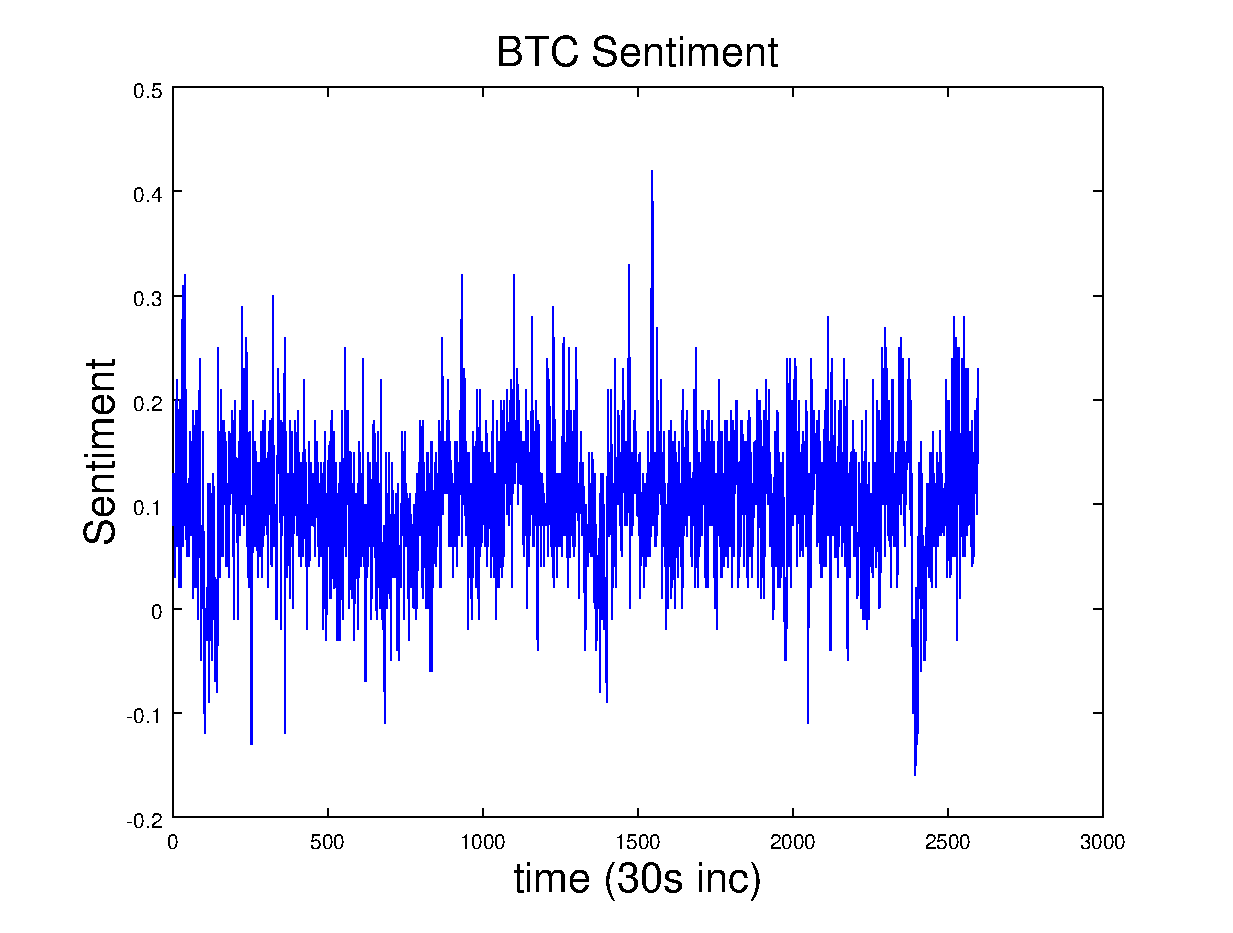
\includegraphics[width=0.5\textwidth]{../Datasets/Plots/Oct9_Sen}
	\caption{Raw Sentiment, October 9th 2017}
	\label{fig:RawSent}
\end{figure}

After a little filtering Figure \ref{fig:FilteredSent}. From here it was possible to compare to time series plots of the
value.

\begin{figure}[h]
	\centering
	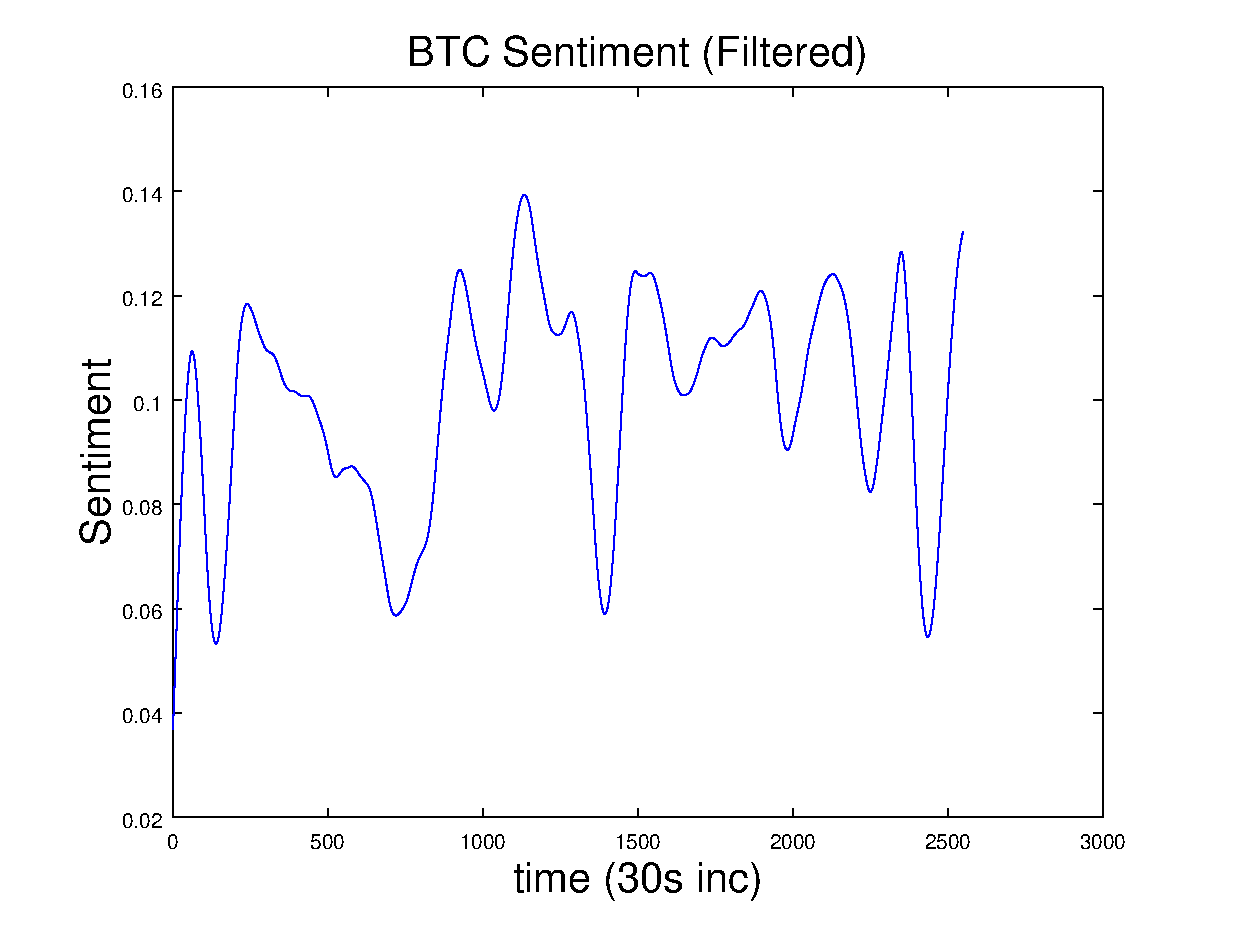
\includegraphics[width=0.5\textwidth]{../Datasets/Plots/Oct9_Sen_Fil}
	\caption{Filtered Sentiment, October 9th 2017}
	\label{fig:FilteredSent}
\end{figure}

\subsection{Timewise Correlation}
The timewise correlation was done by what I call the time correlation vector $k$ which is defined as equation \ref{eq:K}

\begin{equation}\label{eq:K}
k_j = \sum\limits_{i=1}^n x_i - y_{i+j} \textrm{, where j runs from 0 to n}
\end{equation}

\begin{figure}[h]
	\centering
	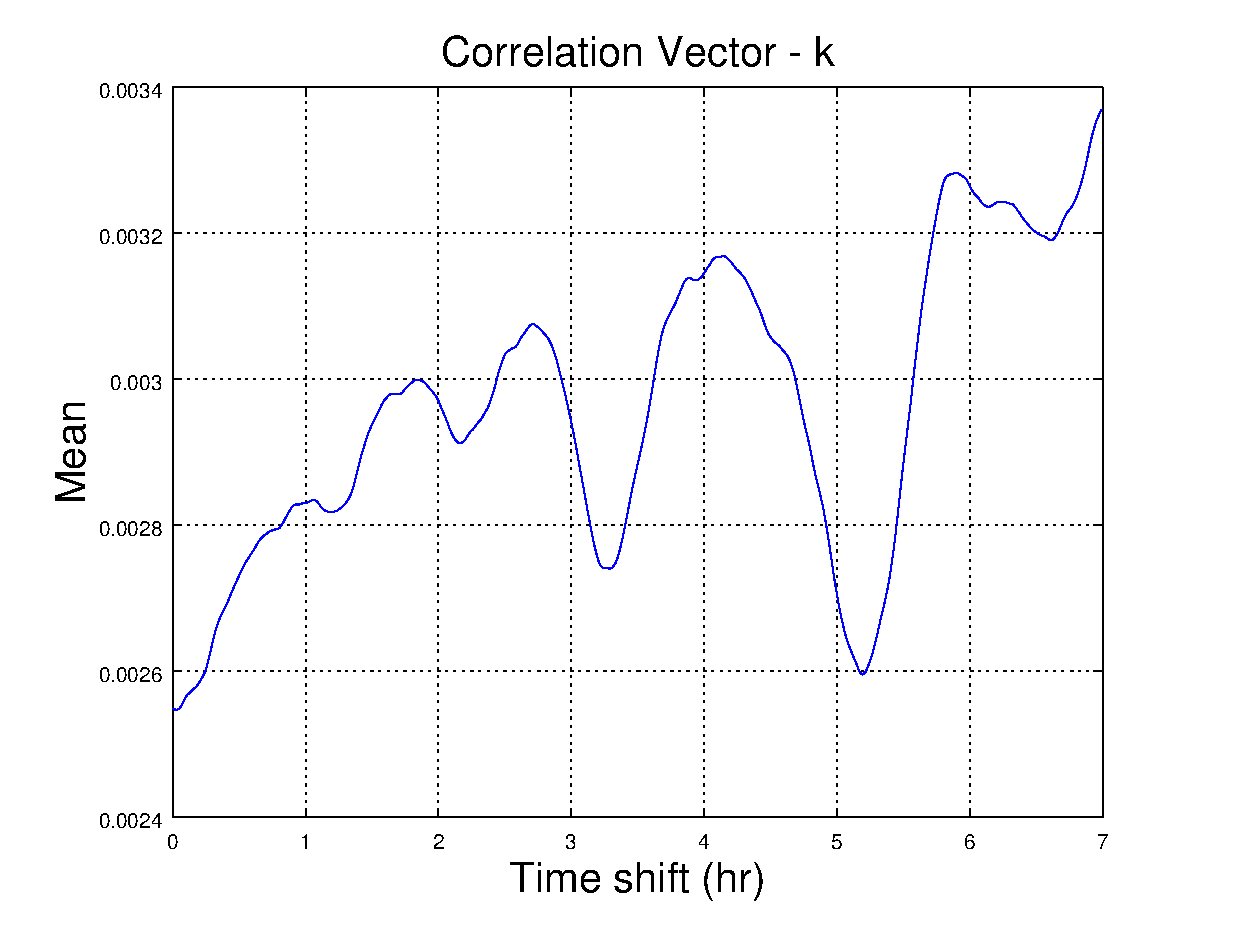
\includegraphics[width=0.5\textwidth]{../Datasets/Plots/Oct7_K}
	\caption{Time Correlation vector $k$,October 7th 2017}
	\label{fig:K}
\end{figure}

Where $x = \frac{dCost}{dt}$ $y = \frac{dSent}{dt}$, the reasoning for using derivatives for the correlation is simply because
the sentiment values are effectively a floating value - where the magnitude is not believed by myself to have any direct 
relationship to the magnitude of cost. However, my findings have lead me to believe that a changing value of sentiment
will induce a changing cost.\\

$k$ is a minimizing function where the lowest magnitude indicates the highest level of correlation.
As seen in Figure \ref{fig:K}, $k$ has a global minima around 5.2hrs, which I define as $\tau_L = 5.2hrs$ 
or the effective 'Time lag' between high values of changing sentiment and high values of changing cost. Figure 
\ref{fig:SentShift} shows the sentiment shifted forward in the by $\tau_L$.

\begin{figure}[h]
	\centering
	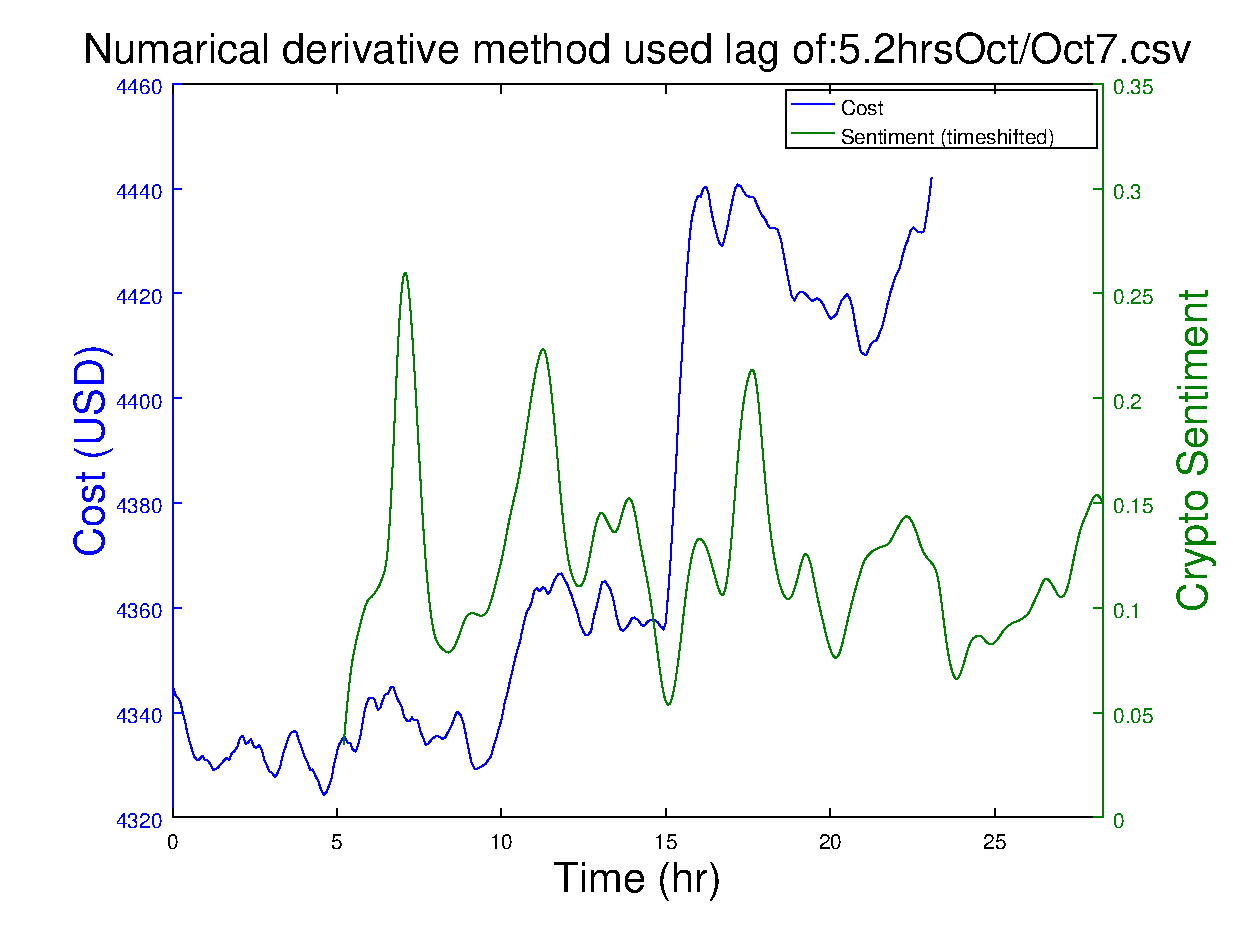
\includegraphics[width=0.5\textwidth]{../Datasets/Plots/Oct7_CostSen}
	\caption{Time Shifted Sentiment, October 9th 2017}
	\label{fig:SentShift}
\end{figure}

It can be observed that rates of high change and local minima and maxima are matched between the two datasets.

\subsection{Realtime Implementation}
Write things here... Maybe?

\section{Conclusion}
The conclusion goes here.

\begin{thebibliography}{1}

\bibitem{BI1}
Anshul Mitta and Arpit Goel, \textit{Stock Prediction Using Twitter Sentiment Analysis}
\end{thebibliography}

\end{document}
